% =========================================================================
% Vent-Snap 棘轮 —— 中文对照版(供内部审阅/交流;投稿以英文 main.tex 为准)
% 与 main.tex 的 09-01 稿(读者视角修订版)逐节对应:数字/公式/引文/图表完全一致,仅语言不同。
% ⚠ 改英文版后中文版不会自动同步——同步义务见 paper/README.md。
% 编译:tectonic main_zh.tex(XeTeX;需系统装有 Noto Serif/Sans CJK SC,
% 本机已放 ~/.fonts;Overleaf 选 XeLaTeX 编译器并上传字体或改用其自带思源)
% =========================================================================
\documentclass[journal]{IEEEtran}

\usepackage{amsmath,amssymb}
\usepackage{graphicx}
\usepackage{booktabs}
\usepackage{multirow}
\usepackage{xcolor}
\usepackage[colorlinks=true,allcolors=blue!60!black]{hyperref}
\usepackage{xeCJK}
\setCJKmainfont{Noto Serif CJK SC}
\setCJKsansfont{Noto Sans CJK SC}

\renewcommand{\figurename}{图}
\renewcommand{\tablename}{表}

% 草稿待办标记——投稿前剥除(与英文版同步)。
\newcommand{\TODO}[1]{\textcolor{red}{\textbf{[待办:#1]}}}

\newcommand{\dstar}{\delta^{*}}

\begin{document}

\title{Vent-Snap 棘轮:吸盘爬壁机器人密封破裂滑移的\\
量化、建模与免力传感消除}

\author{Shaopeng~\TODO{完整作者名单、单位、资助}%
\thanks{中文对照版,供内部审阅与交流;正式投稿版本为英文 main.tex。}%
\thanks{作者单位:\TODO{单位}。联系:\TODO{邮箱}。}}

\markboth{IEEE Robotics and Automation Letters(中文对照版,非投稿稿)}%
{Shaopeng \MakeLowercase{\textit{et al.}}: Vent-Snap 棘轮}

\maketitle

% =========================================================================
\begin{abstract}
以真空吸盘攀爬的腿式机器人每走一步都必须破坏一次密封。我们在柔性、
位置控制的平台上证明:密封破裂会释放腿链中储存的弹性能——机体在几十
毫秒内下坠,随后的再吸附把损失锁定,于是一台零净指令原地踏步的机器人
沿墙棘轮式下滑。用低成本手机视频管线(归一化互相关追踪、逐组米制比例、
指令标记对时),我们把该效应量化到毫米级与逐腿分辨率:每周期位置损失
的 $93\%$ 发生在密封破裂处,每次坠落在两帧视频($\le67$\,ms)内完成。
一维并联弹簧模型解释了损失,
并给出四条经实验验证的预言,其中包括破裂弹跳对放气前预先施加的卸载
位移严格线性。据此我们提出\emph{零力交接}:在一条腿放气之前,把它的
足端沿墙向上指令一个逐腿标定量 $\delta_j$——即该腿链已储存的变形量——
同时把各支撑足沿墙向下指令同样的总量,按"离自己下次抬腿越远份额越大"
的权重分摊,使机体的指令位置保持不变。整个方案纯运动学、纯开环:卸载量
来自离线标定表,不用力/触觉/电流反馈;吸附时序本就依赖的吸盘气压传感器
在交接中不起作用。在 $n{=}3$ 拉丁方实验中,它把总下滑削减
$43\%$(仅 $\delta$)与 $61\%$(加权重),破裂瞬间的下滑削减
$82\%$/$88\%$(配对 $p\le0.0022$)。一项预登记的速率判别实验表明,交接
过程中的残余损耗随转移的位移量而非耗时增长($\Delta b=\kappa\,\delta_j$,
$\kappa$ 跨五天复现至 $4\%$),据此确认剩余的杠杆是载荷份额分配而非
速度($\kappa$ 被权重压低 $44\%$)。数据、日志与量化管线全部开源。
\end{abstract}

\begin{IEEEkeywords}
爬壁机器人,腿式机器人,柔顺与阻抗控制,标定与辨识,机构设计。
\end{IEEEkeywords}

% =========================================================================
\section{引言}
\label{sec:intro}

以真空吸附攀爬的腿式机器人,必须做一件轮式与滑动吸附爬壁机所回避的事:
每走一步都要摧毁一个吸附接触,再在别处重建。对负压足而言,这种摧毁不是
渐进的:被放气的吸盘在残余真空尚存时仍然抓着墙,直到唇口剥离的一瞬才
整体松脱——一种\emph{破裂型}脱附,它把释放一个承载接触的全部力学后果
压缩进几毫秒之内,远低于任何步态控制器的控制带宽。

在刚性机器人上这无关紧要。但小型爬壁平台并不刚:安全余量是用轻量化
3D 打印腿链、顺应表面的波纹吸盘、以及无力矩反馈的低成本位置舵机换来的。
在这样的平台——一台每只脚装一个吸盘的六足步行机器人
(图~\ref{fig:platform})——上我们观察到:命令它在竖直玻璃上
\emph{原地踏步}——一次抬一只脚、再放回原位——时,它每个步态周期沿墙
下滑 $57$--$74$\,mm,尽管吸附中的吸盘在玻璃上从不打滑、六足全部吸附时
机体也从不漂移。逐帧分解显示,本文 $n{=}3$ 实验中 $93\%$ 的损失发生在
密封破裂处(\emph{首次发现实验}——即我们最早观察到该现象的那一组,分段
窗口取得更宽——为 $83\%$);每次破裂坠落在两帧视频($\le67$\,ms)内
完成,而破裂之前的主动放气期间机体位移不足 $0.15$\,mm。机理是弹性的:吸附的脚待在原地,机体却在自重下
下沉,于是每条吸附腿链——脚与机体之间的打印连杆、关节和舵机齿轮系——
像一根受载弹簧一样被拉长;对一条带载腿放气,等于在满张力下剪断这根
弹簧——机体坠落,直到其余腿的额外拉长接住它,而下一次吸附在机体当时
悬停的位置抓住墙,把新位置锁死。我们把由此形成的阶梯式下降称为
\emph{vent-snap 棘轮}。舵机电流佐证了这幅图景:十八只舵机的总线总电流
在两个周期内从 $0.7$\,A 台阶式爬升到 ${\sim}1.9$\,A 且不回落,表明
腿间内力在持续累积。

这一失效组合——柔性支撑链、破裂型脱附、以及会累积内力的位置域驱动
\cite{gorner2009dlr}——对低成本吸附爬壁机是通用的,然而我们没有找到
任何对由此造成的整机位置损失的量化先例(第~\ref{sec:related} 节)。
已有的脱附扰动研究测的是足端力或机体振动,并用力传感器闭环管理;
经典行走机文献中抬腿前的卸载全部在力域执行。我们的平台没有任何力、
触觉或逐关节电流传感,而加装它们会增加重量、走线与复杂度,这对爬壁
机器人而言代价很高。

我们转而利用让这个问题变得可解的唯一事实:吸附的脚不会滑,所以
\emph{改它的位置指令改的是力,不是位置}。于是"只抬无力之腿"这一卸载
条件可以从力域换算到位移域、并纯开环执行:放气之前,把腿 $j$ 的足端
沿墙向上指令一个逐腿常数 $\delta_j$(即其储存变形,由破裂弹跳的线性
外推离线标定)——脚本身动不了,这一指令的效果是把腿这根弹簧松掉;
同时把各支撑足沿墙向下指令同样的总位移、按权重分摊,使六足指令的
均值——从而机体的指令位置——保持不变。我们称之为\emph{零力交接}
(图~\ref{fig:platform}c)。

本文贡献如下:
\begin{enumerate}
\item \textbf{Vent-snap 棘轮的发现与量化。}据我们所知,首次对腿式吸附
爬壁机器人在真空密封破裂瞬间的整机位置损失做出时间分辨、逐腿、毫米级
的量化,并附可复现的低成本视频管线与公开数据。已有的脱附扰动报道对
机体运动只有定性描述,或量化的是足端力、加速度、腔压等其他口径
\cite{kim2008smooth,pei2023review,pan2005suction}。
\item \textbf{带被验证预言的并联弹簧解释。}一维弹性模型解释了损失,
预言破裂弹跳对放气前施加的卸载位移严格线性(已验证;逐腿斜率相差 $4$ 倍,由此得到
的刚度估计与独立路径吻合,$r=0.938$),预言载荷权重的稀释效应(模型
$-32\%$ vs 实测跨指标 $-30$ 至 $-36\%$),并经一项预登记判别实验得到转移损耗
定律 $\Delta b=\kappa\,\delta_j(1+0.20(r{-}1))$($r$ 为步态周期序号)
——其中时间不起作用。
\item \textbf{免力传感、开环、纯软件的解法与 $n{=}3$ 实证。}零力交接
把脱附前卸载——其力传感闭环形式已有先例
\cite{cutkosky2010patent,nadan2024loris}——换算到位移域:逐腿离线标定、
均值不变分摊、轮转权重,卸载回路中不含任何传感器(吸盘气压只用于吸附
时序,与基线相同)。玻璃墙上的拉丁方
$n{=}3$ 实验中,每周期总滑移下降 $43\%$/$61\%$,破裂段滑移下降
$82\%$/$88\%$(三组两两比较 $p\le0.0022$,过 Bonferroni 校正)。
\end{enumerate}

所有优先权主张均以"据我们所知"为限,并在第~\ref{sec:related} 节逐一
对最近邻先例划界。日志、视频、核对图与分析管线将全部公开
\TODO{打包开源数据包;补仓库地址}。

% =========================================================================
\section{相关工作}
\label{sec:related}

\subsubsection{平台谱系}腿式吸附爬壁机按吸附原理分三线:真空/负压足
\cite{hirose1991ninja,zhang2006sky,guan2013wclimbot,li2025biped}、
干粘附/仿壁虎
\cite{unver2006geckobot,kim2008smooth,henrey2014abigaille}、
抓握/微刺足 \cite{parness2017lemur,nadan2024loris};综述见
\cite{nansai2016survey,tao2023climbing}。本文属于最老的一线——离散
步态吸盘足,每一步都要破坏并重建密封;滑动吸附
\cite{longo2004alicia,yue2024snail} 以持续供能为代价回避了这笔账。
我们的平台是这一谱系中的低成本、每腿 3 自由度六足。

\subsubsection{脱附扰动:已被测量的是什么}释放一只粘附足会扰动机体,
这在定性层面早为人知:Stickybot 的设计者报告,各向同性胶垫时代巨大的
脱附力"produc[ed] oscillations that frequently caused the other feet
to slip"(引发振荡,频繁导致其余足打滑)\cite{kim2008smooth};近期
中文综述把"瞬态与较大的脱附力传递到躯干引起机体震颤"列为待攻关问题
\cite{pei2023review}。被\emph{量化}过的都在足端层面:剥离角阻抗控制
降低法向脱附力 \cite{wang2021compliant},旋转剥离把拉脱力削减
$65.5\%$ \cite{wen2025force},轨迹/力整形把最大脱附力降 $28\%$、
IMU 振动降 $82\%$ \cite{xiao2025ftfof}。我们明确指出:
\cite{xiao2025ftfof} 的 $82\%$ 是加速度幅值(m/s$^2$),与本文破裂段
\emph{位移}(mm)削减 $82\%$ 只是数字巧合,量纲无关。真空谱系中我们
找到的唯一瞬态量化是腔压 \cite{pan2005suction}。而每次脱附事件的整机
位置损失——真正决定爬行进度上限的量——在我们能检索到的文献中无一
先例。

\subsubsection{脱附前卸载}抬脚前先卸载的思想有力域、闭环的先例,本文
据此划定自己的主张范围。Stickybot 专利描述了抬离前沿切向卸载、以松弛累积的力
与弹性变形,由霍尔力传感器在刚度控制回路中执行
\cite{cutkosky2010patent};LORIS 的步态状态机含显式 \emph{Unload} 步,
在在线力优化中把待离爪的接触力约束为零 \cite{nadan2024loris};
LEMUR~3 以每肢力传感器管理吸放力 \cite{parness2017lemur};导纳控制在
仿真中缓解肢式攀爬的反力扰动 \cite{imai2024admittance};反力感知规划
整形摆动惯性 \cite{ribeiro2023ramp};准静态步态优化在规划层再分配
接触力 \cite{boscariol2013optimal}。以上全部在力域、闭环或规划层执行,
且无一量化机体滑移。据此本文的主张限定为:把卸载条件换算到
\emph{位移域}(逐腿离线标定、均值不变分摊),在\emph{完全没有力传感}
的平台上\emph{纯开环}执行,并以\emph{破裂段滑移}量化验证。

\subsubsection{行走机力分配经典带}让腿力在抬离前平滑归零,是自
Waldron 的力/运动管理以来的行走机经典课题
\cite{waldron1986force,kumar1988force,klein1990optimal,zhou2000fricom,
erden2007torque},一直延伸到现代全身控制器与 MPC
\cite{righetti2013optimal,bellicoso2016perception,focchi2017high,
dicarlo2018dynamic}。整条带全部在力域执行:或由力/力矩传感器闭环
\cite{gorinevsky1990force,gorner2009dlr},或把力设定值交给能跟踪力的
驱动层。Chen 等的"不需要力传感器"\cite{chen1999optimal} 仅指设定值
计算。DLR Crawler 一文提出了本文所处理的问题——位置控制的多足机器人
会累积内力——并用关节力矩传感解决 \cite{gorner2009dlr}。昆虫也面对
同一问题:载荷向邻腿转移使本腿被机械卸载,由载荷感受器触发摆动
\cite{dallmann2017load}——一个生物学闭环,而我们的开环标定表替代了它。
在这一经典框架下,本文的贡献是为这一经典需求提供了新的执行域,覆盖了
经典解法不适用的平台类别(业余位置舵机、强串联柔性)。

\subsubsection{位移域前馈补柔性}"标定后前馈"补偿结构柔性本身是成熟的
方法族:TITAN~XI 预标定腿系柔性以恢复斜坡落足精度 \cite{doi2005titan};
Ota 等在吸附四足上补偿重力变形以求动作顺滑 \cite{ota2006deformation};
加工机器人用离线刚度模型修正指令轨迹
\cite{wang2009machining,klimchik2014compliance};腿式人形前馈脚底/
关节变形 \cite{takenaka2005floor};仿壁虎爬壁机用刚度模型做重力补偿
以保姿态 \cite{wang2024gecko};sway compensation 在静步态中用位移预移
转移\emph{重力}载荷 \cite{kurazume2002feedforward}。数学形态相同、
目标不同:无一用标定位移去\emph{清零一条即将脱附之腿的内力},也无一
面对被压缩进毫秒的能量释放。

\subsubsection{替代路线}可以避免破裂(滑动吸附 \cite{yue2024snail},
代价是持续供能);可以从电机电流估计接触力 \cite{wahrburg2018motor}
(在齿轮摩擦巨大的业余舵机上不可行,见第~\ref{sec:discussion} 节);
也可以利用 snap-through 储能释放做推进而非承受其扰动
\cite{tang2020spine}。定向干粘附靠材料设计实现近零力脱附
\cite{kim2008smooth,autumn2006frictional};真空吸盘没有这种机制,
因此储能必须\emph{在破裂前归还}。至于直觉上的"慢慢放气",
在我们的数据上并不奏效(第~\ref{sec:ratchet} 节)。

% =========================================================================
\section{平台、管线与现象}
\label{sec:phenomenon}

\subsection{平台}
\label{sec:platform}

实验平台(图~\ref{fig:platform})是一台由开源 MakeYourPet 六足
套件~\cite{makeyourpet2022hexapod} 衍生的 3D 打印六足步行机器人(机身与 coxa/femur 连杆为套件打印件),
配自研打印的小腿—吸盘一体足与气动舱。机器人面朝墙的上方攀爬;腿以
L/R 记左右、以 $1/2/3$ 记从前到后,因此 L1、R1 是最上方的一对,L3、R3
最下方(图~\ref{fig:platform}a)。每条腿有三个位置控制关节
(coxa/femur/tibia 连杆 $43/81/124$\,mm,为实测值、运动学即按此计算),
末端是一只 30\,mm 波纹吸盘。每足一只常闭三通电磁阀把吸盘接向泵歧管
(吸附;断电即此态,失电安全)或接向大气(放气),歧管与阀之间每足一只
单向阀使各吸盘互不串气。本文报告的所有实验均未装储气罐:一台隔膜泵
直接抽歧管,并按吸盘压力读数以砰砰滞环把已吸附吸盘中最浅的一只维持在
$-60$ 至 $-75$\,kPa(任一吸盘正在抽真空时泵无条件运转);低于
$-30$\,kPa 并保持 $0.2$\,s 判吸附成功;仅当其余五盘全部吸附且深于
$-50$\,kPa 门槛时才允许抬腿。步态一次只动一条腿:任一时刻五只脚吸附、
至多一只脚离墙。十八只 35\,kg$\cdot$cm 位置控制业余舵机(无任何力矩、
力、触觉或逐关节电流反馈)由树莓派~Pi~5 经 RP2040 舵机板(运行开源固件~\cite{carrera_chica})驱动;整机质量
$3.54$\,kg。机器人的传感器只有两类:六路吸盘
压力传感器(每足一只),由吸附状态机用于吸附/放气确认、漏气判定、抬腿
门槛与泵滞环;以及舵机板的母线电压/电流遥测,只用于欠压停机与记录。
没有 IMU,足底触点开关未启用,舵机无位置回读。这些读数没有一个进入
交接的计算(第~\ref{sec:method} 节)。全部实验在竖直玻璃上进行,全程
安全绳。平台的柔性不是偶然:打印腿、波纹吸盘与舵机齿轮系共同使机体到
足端锚点的链条软到指令机体位移只有 $42\%$ 被实现
(第~\ref{sec:finding2} 节)——这正是该级别机器人所必需的轻量化构造的
典型特征。

\begin{figure}[t]
\centering
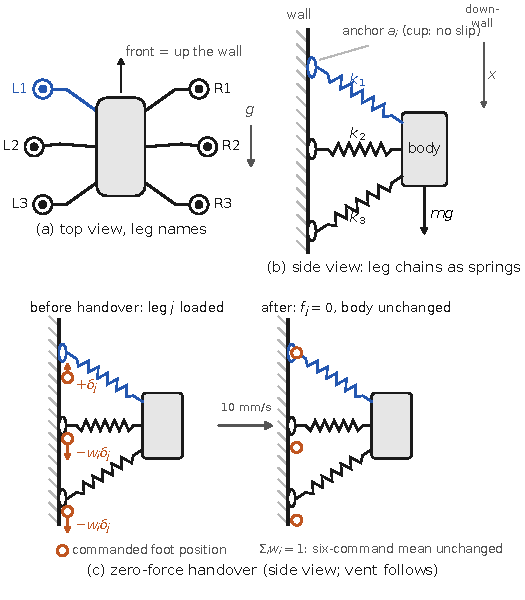
\includegraphics[width=\linewidth]{figures/fig_platform.pdf}
\caption{平台与零力交接(示意图)。(a)~俯视与腿命名:机器人面朝墙的
上方,故 1 号腿为最上方一对。(b)~侧视:每条吸附腿链相当于机体与足端
锚点 $a_i$(不会打滑)之间的一根弹簧 $k_i$;机体在自重 $mg$ 下挂在
这些弹簧上;$x$ 沿墙向下计量。(c)~零力交接,以一条上方腿 $j$ 为例:
吸附中的脚都位于各自指令位置(空心圆)的上方,即每条腿都被拉长。放气
$j$ 之前,其足端指令沿墙向上移动 $\delta_j$ 直到弹簧松弛($f_j=0$),
各支撑足指令同时沿墙向下移动 $w_i\delta_j$、$\sum_i w_i=1$;机体的
指令位置不变,随后密封断开时已无可释放。\TODO{补 (d):机器人在玻璃墙上
的照片。}}
\label{fig:platform}
\end{figure}

\subsection{量化管线}
\label{sec:pipeline}

机体沿墙位置由固定手机相机(4K@30\,fps)测得:对机身电路板做归一化
互相关(NCC)模板追踪,亚像素抛物线插值,并以画面静物参照块逐帧扣除
相机抖动。米制比例\emph{逐组}标定:取机身上刚性安装的一块 PCB 的长边
($93.0$\,mm),四角亚像素定位(各组 $0.288$--$0.296$\,mm/px;顶边与
底边长度相差 $1.1$--$2.7\%$,比例取两者均值)。视频与机载事件日志的对时用指令
标记——\emph{机体倾身}:每组开始时,在六足全部吸附的状态下命令机体
沿墙向上 $10$\,mm 再回来,把指令曲线与追踪轨迹做形状拟合(各组 $R^2$
$0.95$--$1.00$);同一标记兼作柔性探针(第~\ref{sec:finding2} 节)。
随后把每次抬落按时间顺序分解为五段:\emph{交接}(放气前的位移转移,
见第~\ref{sec:method} 节,启用时)、\emph{vent}(基线组从阀开指令前
$1$\,s 起,交接组从阀开指令本身起——它同时是交接段的终点——到日志
"释放确认"事件后 $0.4$\,s 止;释放确认 = 吸盘压力回升到 $-5$\,kPa
以上,下文称"盘压归零";该窗包含密封破裂,其中累计的下滑称为
\emph{破裂段滑移})、\emph{摆动}(脚在空中)、\emph{落地压入}、
\emph{静置}。分段之和与人工皮尺读数核对过(首次发现实验:追踪
$131.3$\,mm vs 人读 $131$\,mm);全部比例板与模板锁定经人工对 188 张
存档核对图核查。

\subsection{Vent-snap 棘轮}
\label{sec:ratchet}

原地踏步能把该效应单独分离出来:按固定的\emph{轮转}序
(R3$\to$L1$\to$R2$\to$L3$\to$R1$\to$L2;六条腿各抬一遍称为一
\emph{轮},即一个步态周期)逐腿抬到指令高度玻璃面上方 $15$\,mm
(足端指令行程 $33$\,mm,因为吸附态指令压在玻璃面下 $18$\,mm 作预压)、
悬停 $1$\,s、放回名义站位;指令的机体净位移为零,因此任何系统性位移
只能来自弹性应变的释放与再锁定。两项对照验证了前提:操作者核对的
吸附盘旁玻璃标记全程不动(吸盘不打滑),六足全部吸附期间机体不蠕变
(静置段在三轮一组中合计仅 $2.4$--$4.7$\,mm;另见
第~\ref{sec:mechanism} 节)。然而机体每周期下降 $57$--$74$\,mm
(首次发现实验;$n{=}3$ 基线为 $63.9\pm0.9$\,mm,
第~\ref{sec:results} 节),阶梯的每一级都与一次密封破裂重合
(图~\ref{fig:staircase})。

\begin{figure}[t]
\centering
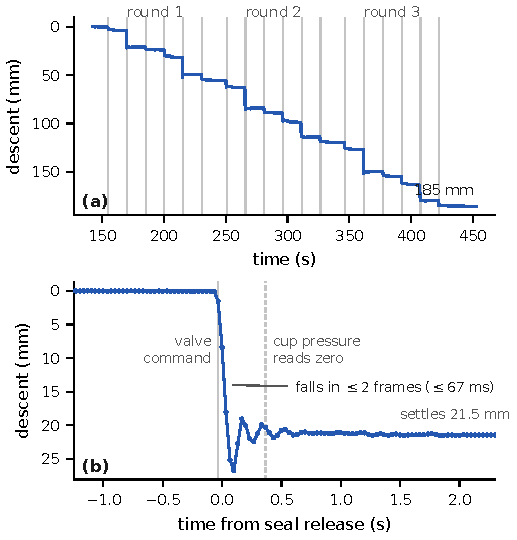
\includegraphics[width=\linewidth]{figures/fig_staircase_zoom.pdf}
\caption{Vent-snap 棘轮(基线,重复 \#1)。(a)~三轮原地踏步的机体沿墙
位置:$185$\,mm 阶梯的每一级都与一次密封破裂(灰线)重合,级间轨迹
平坦。(b)~一次抬落(L1,第 2 轮)的原生 30\,fps 剖面,$t{=}0$ 取追踪
到的释放时刻:释放前机体纹丝不动,两帧内坠 $21.5$\,mm 并带欠阻尼过冲
(峰 $26.7$\,mm);同一瞬间被释放的脚沿墙回弹 $12.8$\,mm(图中未示)。
日志的阀开指令与释放确认(盘压归零)两事件夹住机械释放;两者相对视频的位置带
对时不确定度(零点几秒)。}
\label{fig:staircase}
\end{figure}

有三个时间尺度。(i)~放气指令后残余真空排出期间,机体不动
($<0.15$\,mm)。(ii)~密封破裂时,全部下坠在 $1$--$2$ 帧
($33$--$67$\,ms)内完成,带欠阻尼过冲(图~\ref{fig:staircase}b:峰 $26.7$\,mm、稳于
$21.5$\,mm)——典型的弹性释放特征。(iii)~事件之间轨迹平坦。$n{=}3$
基线中 vent 段合计 $172.9\pm3.4$\,mm,占总量 $185.5\pm3.0$\,mm 的
$93\%$;落地压入占 $4\%$(首次发现实验的分解为 $83\%$/$4\%$,其再平衡
窗口取得更宽)。被释放的脚在同一瞬间沿墙向下回弹 $9$--$15$\,mm
(下限:追踪块含一段腿节)。逐腿单次弹跳最大 $20.9$\,mm(L1)与
$19.2$\,mm(R1)——最上方的一对,机体自重对吸盘的剥离力矩在此最大
——而最软的中间一对(L2/R2)仅 $3.5$--$6.1$\,mm,这是腿链刚度强烈
不均的第一个信号。

两条推论约束了设计空间。第一,\emph{慢放气无济于事}:数据显示残余
真空排出期间机体零位移,说明力并不是随压力衰减逐渐释放的,而是在唇口
剥离的一瞬一次放完;放得再慢也只是把同一级台阶往后推。(我们没有直接
测试更慢的放气;这一推断依据的是破裂前的平坦轨迹与不打滑对照。)因此
任何解法都必须保证\emph{密封松脱那一刻}这条腿本来就不带力。第二,损失被下一次吸附锁定:新鲜吸盘在机体当时所在的位置以
零预载抓住墙(第~\ref{sec:model} 节),于是每次下坠累积成棘轮而不会
自行平均掉。舵机总线电流反映了同样的累积:从首次全吸附的
$0.73$\,A 起台阶式爬到两周期后的 ${\sim}1.9$\,A 且不回落——每锁定
一级下坠,支撑腿承受的内力就增加一份。

% =========================================================================
\section{并联弹簧解释}
\label{sec:model}

\subsection{模型}

把每条吸附腿链 $i$ 沿墙面重力轴($x$ 向下为正;图~\ref{fig:platform}b)
折叠为一根刚度 $k_i$ 的线性弹簧。设 $a_i$ 为足 $i$ 的(不动)锚点,
$c_i$ 为控制器给该足的指令位置(相对机体表示),定义
$y_i \equiv a_i - c_i$:即脚恰好处在指令位置、腿 $i$ 零受力时的机体
位置。
腿 $i$ 对机体施加剪切力 $f_i = k_i\,(x - y_i)$(沿墙向上为正),
吸附集 $S$ 的静力平衡给出
\begin{equation}
x \;=\; \langle y\rangle_k + \frac{mg}{K},
\qquad
\langle y\rangle_k \equiv \frac{\sum_{i\in S} k_i y_i}{K},\;\;
K \equiv \sum_{i\in S} k_i .
\label{eq:equilibrium}
\end{equation}
机体悬在各腿零力位置的\emph{刚度加权}平均之下。三类事件驱动动力学:

\emph{零预载锁定。}密封形成的吸盘在机体当前位置抓墙、不储力:
吸附即置 $y_j \leftarrow x$。

\emph{破裂。}对腿 $j$ 放气,等于移走一根带张力 $f_j$ 的弹簧;机体
坠至接住集的新平衡,
\begin{equation}
b_j \;=\; \frac{f_j}{K - k_j},
\label{eq:bounce}
\end{equation}
即\emph{观察到的弹跳是这条腿储存的力除以其余腿的并联刚度}——不是
它自己的储存变形 $e_j = f_j/k_j$。比值 $e_j/b_j = (K-k_j)/k_j$
(六腿等刚度时为 $5$)在本平台从最硬腿的 $1.7$ 到最软腿的 $8$
(第~\ref{sec:calib} 节),这一区别对标定至关重要。

\emph{加载。}从吸附到抬起之间,机体每下沉一毫米,每条吸附腿就被多
拉长一毫米($x-y_i$ 增大);吸附得越早的腿被拉得越长,同样指令下各腿
储力互不相同。

把锁定、加载、破裂沿步态在一维仿真中迭代即重现棘轮:稳态原地损失约为
每周期 ${\approx}0.4\,mg/\bar{k}$,与实测 $74$\,mm/周期匹配得整机
柔度尺度 $mg/\bar{k}\approx185$\,mm。硬腿弹跳在 ${\sim}20$--$27$\,mm
处进入平台、第 2 轮之后不再增长,而 $mg/\bar{k}=185$\,mm 的线性模型
会高估前进爬行的损失(它预测净倒退,实测却净挣 $+26\%$ 的指令步幅);
我们把这两点都归因于舵机扭矩饱和给单腿可储能量封了顶——这是假说,
不是测量 \TODO{净前进率 demo(T4b)完成后刷新此数}。

\subsection{四条被验证的预言}
\label{sec:predictions}

\emph{P1:破裂弹跳对放气前施加的卸载位移严格线性,斜率编码腿刚度。}
若放气前把腿 $j$ 的足端沿墙向上指令 $\delta$、即把 $y_j$ 朝 $x$ 移动
$\delta$(第~\ref{sec:method} 节),残余张力
减少 $k_j\delta$,故 $b_j(\delta) = b_j(0) - s_j\,\delta$,其中
$s_j = k_j/(K-k_j)$。三剂量标定实验($\delta = 0/12/24$\,mm,六腿同值;
第~\ref{sec:calib} 节,图~\ref{fig:linearity})显示六腿全部严格线性
(中点残差 $\le1$\,mm),斜率 $0.13$--$0.57$——$4$ 倍的逐腿散布直接
量出了刚度不均。由斜率归一化的刚度 $\hat{k}_j = s_j/(1+s_j)$ 与一条
完全独立的第二路径(拟合交接段下沉,第~\ref{sec:mechanism} 节)吻合,
Pearson $r=0.938$。

\emph{P2:新吸附的腿几乎不弹。}零预载锁定意味着刚吸附之腿的第一次
抬起只释放锁定以来累积的力:每组基线的首抬(R3)都是该腿最小的一次
弹跳——无起跑标记的两组为 $-0.0$ 与 $+1.8$\,mm,主实验三组基线(首抬
前多了 $\pm10$\,mm 标记)为 $2.5$--$4.3$\,mm——而后续轮次随加载累积
升到 $6$--$8$\,mm。

\emph{P3:平衡是刚度加权的,均值不变指令并不能完全冻住机体。}由
\eqref{eq:equilibrium},把 $y_j$ 上移 $\delta$、支撑按权重 $w_i$
($\sum w_i = 1$)下移的交接使平衡点移动
\begin{equation}
\Delta x \;=\; \frac{\delta\,\bigl(k_j - \sum_{i\in S\setminus j} k_i
w_i\bigr)}{K},
\label{eq:redistribution}
\end{equation}
仅在等刚度下为零。卸载\emph{最硬}的腿必然使机体下沉;L1 的一阶预测
(P1 斜率刚度、均分份额)$4.6$\,mm vs 实测 $6.8$\,mm(首轮),而
\eqref{eq:redistribution} 的拟合形式加上 \eqref{eq:fit} 的共模项后,
以 RMSE $0.85$\,mm 重现 B 工况全部 $54$ 个腿$\times$轮$\times$重复
单元(第~\ref{sec:mechanism} 节)。

\emph{P4:载荷份额加权稀释储能。}因为每次锁定都把一条
腿清零,早接到的载荷会被后续锁定部分吸收回集体,晚接到的则原封不动
带进该腿自己的抬起。把交接份额偏向\emph{离下次抬起最远}的支撑腿
(前方稀释机会最多)可降低稳态储能:一维模型给出温和档
($0.35/0.25/0.2/0.15/0.05$)$-19\%$、部署档($0.6/0.25/0.1/0.05/0$)
$-32\%$、温和档反向 $+30\%$(比均分更糟)。实测 B$\to$C 的残余滑移
降幅跨指标为 $-30$ 至 $-36\%$(按总量逐重复为 $-28$ 至 $-33\%$;
第~\ref{sec:results} 节)。

\begin{figure}[t]
\centering
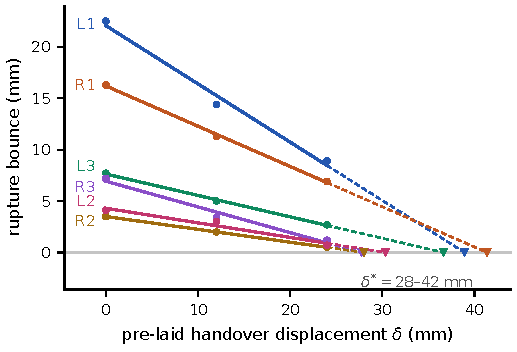
\includegraphics[width=\linewidth]{figures/fig_bounce_delta.pdf}
\caption{P1 验证:破裂弹跳 vs.\ 放气前施加的卸载位移 $\delta$(三剂量
标定第 2 轮,$\delta=0/12/24$\,mm,六腿同值)。六腿全部严格线性(中点残差 $\le1$\,mm);
斜率逐腿相差 $4$ 倍(刚度不均);虚线外推至零弹跳给出标定目标
$\dstar_j=28$--$42$\,mm(三角)。}
\label{fig:linearity}
\end{figure}

% =========================================================================
\section{零力交接}
\label{sec:method}

\subsection{位移域卸载}

解法源自一条不变式:吸附的吸盘不滑(已验证,第~\ref{sec:ratchet} 节),
所以足端指令挪的是力、不是脚。放气腿 $j$ 之前,步态控制器插入
HANDOVER 相位(图~\ref{fig:platform}c):被抬腿的足端指令\emph{沿墙
向上}移动 $\delta_j$(归还其储存变形),每只支撑足指令\emph{沿墙向下}
移动 $w_i\,\delta_j$、$\sum_{i} w_i = 1$(接过载荷);两者都沿墙面的
竖直轴(机器人面朝上方,故即其前进轴)以 $10$\,mm/s 准静态施加。六足
指令均值不变,机体被命令原地不动;被抬腿的力被推到零;随后密封破裂时
已无可释放之物。支撑腿承担的从不超过抬腿\emph{之后}它们本来就要承担
的量——交接只是把移交提前并做成无损。指令保持有界:一个步态周期内
每条腿按份额累计接收约一个 $\delta$ 的向下量,轮到自己抬时归还自己的
$\delta_j$;逐腿的残差在该脚落回名义站位时清零。用部署表仿真指令流,
净效果是首轮累积一次性的六足指令均值偏移(均分份额约 $14$\,mm、轮转
权重约 $20$\,mm,均为指令沿墙向上,按实测传递比折合机体实际上移约
$6$--$9$\,mm),此后均值在 $\pm0.9$\,mm 内摆动、逐轮净漂移为零——
这也是判定不取第 1 轮的原因之一(第~\ref{sec:protocol} 节)。

\subsection{逐腿标定:弹跳不等于储能}
\label{sec:calib}

朴素标定——令 $\delta_j$ 等于观测弹跳——败在
\eqref{eq:bounce} 的系数上:弹跳是储存的力经\emph{其余}腿并联刚度
读出的读数,把储存变形低估 $1.7$--$8$ 倍(因腿而异)。正确且
比例无关的流程由 P1 直接给出:跑三剂量($\delta = 0$、半、全),
逐腿拟合直线,外推到零弹跳截距 $\dstar_j = b_j(0)/s_j$。实测
$\dstar = 28$--$42$\,mm;部署 $\delta_j = 0.8\,\dstar_j$——刻意
留欠:小残余弹跳无害,过冲则会把腿反向预载——得表
L1/R1/L3/R3/R2/L2 $= 31/33/29/22/22/24$\,mm。由于 $\dstar$ 是同量纲
量的比值,它与视频比例标定无关——是本文对比例最不敏感的量。剂量响应
单调($0/12/24$ 下每周期 $65.6\to50.0\to38.7$\,mm),且阶梯性质不变:
$\delta$ 压低的是每级台阶的高度,不是它发生的时刻。

\subsection{轮转距离载荷权重}

P4 决定了分摊:份额按\emph{轮转距离}——即各支撑腿距自己下次抬起还有
几次抬腿——分配:刚抬过的支撑腿(离自己下次抬起最远)拿最大份,下一个
要抬的不拿($0.6/0.25/0.1/0.05/0$,按"最近抬过→下一个要抬"排列)。
控制器每个控制周期对当前支撑集重新归一,且一旦抬腿序偏离轮转即退回
均分并留日志痕——权重假设循环步态,错用会把载荷集中到一条腿。权重改变
稳态运行点;实际上,不开权重标定的表在权重下无需修正,B、C 两条件用的
是同一张表(第~\ref{sec:protocol} 节)。

\subsection{实现与护栏}

方法在步态控制器中约 $150$ 行代码(含注释约 $270$ 行):抬腿决策与
VENT 之间一个新相位、一个逐周期位移更新,无新硬件、不新增传感、除 $\delta$ 表外无
逐机调参。安全护栏(本文所有实验中零触发):某只吸盘真空衰减、自动漏气
挽救程序补抽时,位移转移暂停;每个控制周期的足端目标都经腿工作空间
包络检查,越界则截断交接(部分卸载,留痕)而不是把支撑腿推出工作
空间;转移完成后复检 $-50$\,kPa 抬腿门槛——因为距抬腿决策已过数秒。
交接在部署表下每步增加 $\delta_j/(10$\,mm/s$)\approx2.2$--$3.3$\,s
的周期时间——这是时间上的代价;能耗代价在第~\ref{sec:cost} 节量化。

% =========================================================================
\section{实验}
\label{sec:experiments}

\subsection{协议}
\label{sec:protocol}

\emph{条件。}A:基线原地踏步;B:A $+$ 零力交接(标定表
$\delta_j = 0.8\dstar_j$,均分份额 $w_i = 1/5$);C:B $+$ 轮转距离
权重(同一张 $\delta$ 表)。每个条件只变一个变量。

\emph{设计。}$n{=}3$ 全流程重复,每次重复独立完成三个条件的
上墙—实验—取下,组序按 $3\times3$ 拉丁方(\#1 A$\to$B$\to$C、
\#2 B$\to$C$\to$A、\#3 C$\to$A$\to$B),使条件与场内顺位、电池状态、
玻璃状况解耦。每组:六足吸满后先静置 $21$--$58$\,s(操作者计时;
内建的 $60$\,s 静置是这些组跑完之后才加进启动序列的,适用于
第~\ref{sec:mechanism} 节的 D$'$ 系列),然后一键启动固定自动序列
——$\pm10$\,mm 对时标记、$3$ 轮 $\times$ $6$ 腿抬—悬—放(腿间
$\ge10$\,s 且须泵已停 $\ge2$\,s,实际每个间隔都由 $10$\,s 下限决定)、
轮间 $15$\,s、尾静置 $30$\,s——节奏由构造保证逐组一致。每场电池起点
$\ge7.88$\,V;组内相机不碰(有两场在组间动过,
第~\ref{sec:deviations} 节);比例逐组重标。九组
日志无安全冻结与漏气挽救暂停、无包络截断、无抬腿门槛等待。按协议以第 2 轮
判定(第 1 轮含已知的爬坡与指令复位伪迹,第 3 轮作复核)。

\subsection{主结果}
\label{sec:results}

\begin{table}[t]
\caption{主结果,$n{=}3$ 拉丁方(mm;重复间均值 $\pm$ 样本标准差)。
百分比相对 A。一轮 = 六条腿各抬一遍;破裂段 = vent 窗内累计下滑;交接段
= 放气前位移转移期间的下滑;电流增量 = 组末与组初的舵机总线电流之差。}
\label{tab:main}
\centering
\footnotesize
\setlength{\tabcolsep}{3.5pt}
\begin{tabular}{@{}lrrr@{}}
\toprule
 & A(基线) & B($+\delta$) & C($+$权重) \\
\midrule
第 2 轮下滑 & $63.9\pm0.9$ & $38.1\pm1.0$ & $26.5\pm1.7$ \\
三轮总下滑 & $185.5\pm3.0$ & $105.6\pm2.2$ & $72.9\pm3.0$ \\
 & & $(-43\%)$ & $(-61\%)$ \\
破裂段 & $172.9\pm3.4$ & $31.6\pm1.0$ & $20.1\pm3.3$ \\
 & & $(-82\%)$ & $(-88\%)$ \\
交接段 & --- & $60.2\pm2.2$ & $39.7\pm4.3$ \\
电流增量(A) & $+0.97\pm0.02$ & $+2.40\pm0.08$ & $+1.85\pm0.08$ \\
\bottomrule
\end{tabular}
\end{table}

表~\ref{tab:main} 与图~\ref{fig:waterfall} 汇总了主结果。逐重复配对差
(df $=2$,双侧):B$-$A $=-79.9\pm5.0$\,mm($t=27.9$,$p=0.0013$);
C$-$A $=-112.6\pm5.9$\,mm($t=32.9$,$p=0.00092$);C$-$B
$=-32.7\pm2.7$\,mm($t=21.4$,$p=0.0022$)。三组比较全部通过
Bonferroni 校正($p\times3 < 0.007$)。需要强调这里 $n{=}3$ 的含义:
三次\emph{全流程}独立重复,每次重复每条件含 $18$ 个抬落事件,且相对
效应在重复间几乎恒定(B/A:$-42/-45/-42\%$;C/A:$-61/-63/-58\%$)
——处理效应比实验中任何噪声尺度都大一个量级。拉丁方解耦后未见顺序
效应。

逐腿破裂弹跳(第 2 轮,$n{=}3$):基线重现五天前的首次发现实验
(A 工况 L1 $20.1\pm1.3$ vs $20.9$);C 工况下全腿 ${\le}2.4$\,mm,
基线中贡献最大的两条硬上腿降到 $0.9\pm0.5$(L1)与 $0.9\pm0.3$\,mm
(R1)——在贡献最大的腿上逐腿削减 $95\%$。R1 出现过两次轻微上弹
(约 $-0.9$\,mm,B 工况),即轻度过冲的特征,按宁欠勿过的规则接受。

\begin{figure}[t]
\centering
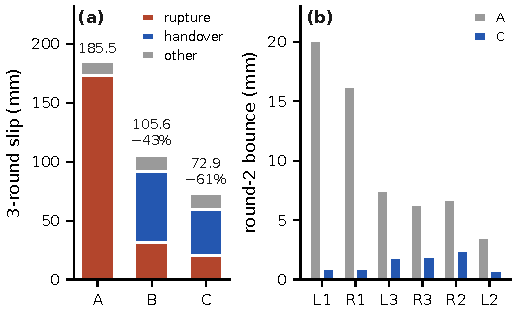
\includegraphics[width=\linewidth]{figures/fig_waterfall.pdf}
\caption{损失的分布($n{=}3$ 均值)。(a)~按段与条件分解的三轮下滑:
交接把 $173$\,mm 的冲击式破裂损失换成 $60$\,mm 的准静态转移损耗;
权重再压到 $40$\,mm。(b)~第 2 轮逐腿破裂弹跳,A vs.\ C:硬前腿从
$20.1$/$16.2$ 降到 $0.9$/$0.9$\,mm。}
\label{fig:waterfall}
\end{figure}

\subsection{发现 1:残余位于转移过程,集中于最硬的腿,且逐轮增长}
\label{sec:finding1}

破裂滑移被压制后,B/C 残余的约一半到五分之三(逐重复 B $56$--$58\%$、
C $47$--$62\%$)落在\emph{交接段},集中于最硬的两条腿,且 L1 逐轮
增长(B 工况 L1:三次重复分别 $6.8\to10.3\to12.6$、$6.9\to8.6\to10.6$、
$6.7\to8.8\to11.9$\,mm;R1 量级相同、$6.6$--$11.4$\,mm,但不单调;
其余四腿 $0$--$2$\,mm)。一阶解读——P3 的刚度加权平衡
——对\emph{形状}正确,但如下文建模所示,对\emph{量级}是错的:
再分配只解释 $60$\,mm 段中的约 $7$\,mm。这笔残余的分解、以及真正
能减小它的因素,是第~\ref{sec:mechanism} 节的主题。

\subsection{发现 2:$42\%$ 的指令—机体柔性传递比}
\label{sec:finding2}

$\pm10$\,mm 对时标记兼作柔性探针:跨 $9$ 个标记、$2$ 天 $3$ 场、$5$ 个
机位,
指令 $10$\,mm 机体倾身实际产生 $4.22\pm0.30$\,mm 机体位移——
\emph{传递比 $42.2\pm3.0\%$},且跨条件不变(A/B/C
$4.15/4.28/4.22$\,mm),符合"探针在全支撑静置态执行"的预期。指令位移
的六成被腿链弹性吸收。我们把它作为平台特性表征而非新发现来报告:
它量化了使棘轮变大的那份柔性,并喂给模型的总增益(下文拟合的
$c_0$)。

\subsection{机理:拟合与一项预登记判别实验}
\label{sec:mechanism}

\subsubsection{交接段拟合}
逐腿逐轮的交接段位移(B:$3$ 次重复共 $54$ 个单元)用
\begin{equation}
\Delta b_{j,r} \;=\;
c_0\,\delta_j\bigl(\hat{k}_j - \textstyle\sum_i \hat{k}_i s_i\bigr)
\bigl(1+\gamma(r{-}1)\bigr) \;+\; \Delta b^{\mathrm{cm}}_{j,r},
\label{eq:fit}
\end{equation}
拟合,第一项即带轮增长因子 $\gamma$ 的 \eqref{eq:redistribution},
第二项是全腿共享的\emph{共模}项。B 组内,模型在 $6.8$--$12.6$\,mm 的
信号上达到 RMSE $0.85$\,mm、留一重复交叉验证 $0.99$\,mm,拟合的
$\hat{k}$ 与 P1 斜率路径在 $r=0.938$ 上吻合(最终联合估计,
$c_0=1.15$:L1 $0.265$、R1 $0.227$、L3 $0.137$、R2 $0.133$、R3
$0.125$、L2 $0.112$;$\gamma=0.11$;由于 \eqref{eq:fit} 只能辨识乘积
$c_0(\hat{k}_j - \sum_i \hat{k}_i s_i)$,$\hat{k}$ 的绝对散布与 $c_0$
互相折换,稳的只是它们的排序与比值)。由此得到的分解推翻了一阶解读:
B 的 $60.2$\,mm 交接段 $=$ 再分配 ${\sim}6.7$ $+$ 共模 ${\sim}55.5$;
C 的 $39.7 = 7.7 + 30.0$(下文的四条件最终拟合给出 $5.7+54.5$ 与
$6.5+33.0$)。\emph{残余的大部分——B 中 $92\%$、C 中 $76$--$84\%$
——是每次交接都要付一遍的共模下沉}——而"集中在硬腿"只是形状效应:软腿上
\eqref{eq:redistribution} 的再分配项为\emph{负}(卸载软腿使机体
微升),恰好抵消共模基座;硬腿上两者相加。

\subsubsection{共模是什么?一项预登记判别}两个假说把 $n{=}3$ 数据
拟合得同样好,因为固定速率下转移时长与转移的位移量完全共线
($T \approx 0.5 + \delta_j/10$):(H1)\emph{时间蠕变}
($\Delta b^{\mathrm{cm}} = \rho\,T$,损耗 $\propto$ 窗时长)vs
(H2)\emph{逐毫米转移损耗}($\Delta b^{\mathrm{cm}} =
\kappa\,\delta_j$)。仅凭观测数据做模型选择无法区分两者:在
$n{=}3$ 数据上两者不可区分($\Delta$AICc${\approx}2$,略偏向 H2),
而我们最初那轮没有 H2 参赛的模型赛马选中的是时间蠕变。唯一的判别
手段是干预:改变转移\emph{速率}。我们在实验协议中
预登记了该实验,上墙之前就写好了两种结果各自的判读表:三对同日
C-vs-D$'$ 配对、顺序交替,D$'$ 与 C 唯一差异是交接位移以 $20$\,mm/s 而非 $10$\,mm/s 施加
(实测交接窗时长 $3.18\to1.83$\,s),预测 H1:交接段
$39.7\to{\sim}26$\,mm(即每组无代价地改善约 $12$\,mm);H2:不变。

\begin{table}[t]
\caption{速率判别(D$'$):预测 vs.\ 结果(每组交接段滑移,mm),
及四条件(B、C、D$'$ 与 C$_{31}$——判别当日的三组对照;$216$ 个
腿$\times$轮单元)联合模型选择。}
\label{tab:dprime}
\centering
\footnotesize
\begin{tabular}{@{}lrr@{}}
\toprule
 & 预测 & 实测 \\
\midrule
H1 时间蠕变($\rho T$) & $26.0$ & \multirow{2}{*}{$36.6\pm1.6$} \\
H2 逐毫米($\kappa\delta$) & $\approx39.5$ & \\
\midrule
\multicolumn{3}{@{}l@{}}{联合拟合($\Delta$AICc,越低越好):
\textbf{H2} $\kappa\delta$:$\mathbf{0.0}$;\; H1 $\rho T$:$17.8$;}\\
\multicolumn{3}{@{}l@{}}{\quad 分条件常数:$31.6$;\;
电流类:$70.6$/$73.0$。}\\
\bottomrule
\end{tabular}
\end{table}

结果(表~\ref{tab:dprime},图~\ref{fig:dprime})很明确:速率翻倍
后交接段仍为 $36.6\pm1.6$\,mm(配对 D$'{-}$C $=-2.9\pm2.1$\,mm,
$p=0.14$;总量 $-1.7\pm0.7$\,mm,$-3\%$),远离 H1 的 $26.0$;从 H2 预测值向 H1 预测值量,结果只走了 $0.21$
的路程;交接段与 vent 段合并比较给出同样不显著的图景
($-3.0\pm3.1$\,mm),其中一对的减少量重新出现在 vent 窗里(快铺下
每次约 ${\sim}1$\,mm 的弛豫尾巴越过了分段边界)。
把每次交接按放气时刻对齐(图~\ref{fig:dprime})直接显示了机理:D$'$
的斜坡陡一倍而\emph{平台完全相同}(L1 全六组 $7.9$--$8.8$\,mm)
——下沉准静态地跟随转移的毫米数,不随窗口时间累积。健全性检查确认
更快的速率没有引入其他变化:逐腿破裂弹跳、传递比
($4.30/4.42$\,mm)、电流增量两条件间均不变。

\subsubsection{转移损耗定律及其决定因素}
四条件联合拟合(H2)把共模定为
\begin{equation}
\Delta b^{\mathrm{cm}}_{j,r} \;=\; \kappa\,\delta_j\,
\bigl(1 + 0.20\,(r{-}1)\bigr),
\label{eq:kappa}
\end{equation}
其中 $\kappa$ 是\emph{载荷份额分配}的属性,与时间无关:均分
$\kappa_B = 0.099$\,mm/mm;轮转权重 $\kappa_C = 0.055$(五天后同
工况复测:$0.053$——$4\%$ 的复现)。为稀释储能(P4)而引入的权重,
实际主要作用是\emph{把 $\kappa$ 压缩了 $44\%$}。机理上,
该定律指向载荷转移期间吸盘/腿链界面的准静态逐毫米损耗(微滑移或
结构非线性)——而不是时间蠕变,与零漂移静置对照一致。实用读法:
位移转移的速度不影响损耗;份额分配是剩余的可调因素;而
${\sim}37$--$40$\,mm 的残余交接段是在当前 $\kappa$ 下每轮转移
$\sum_j\delta_j = 161$\,mm 的固有代价
($\kappa\sum\delta\times3 \approx 26$\,mm $+$ 再分配 ${\sim}6$--$8$
$+$ 逐轮爬坡)。

\begin{figure}[t]
\centering
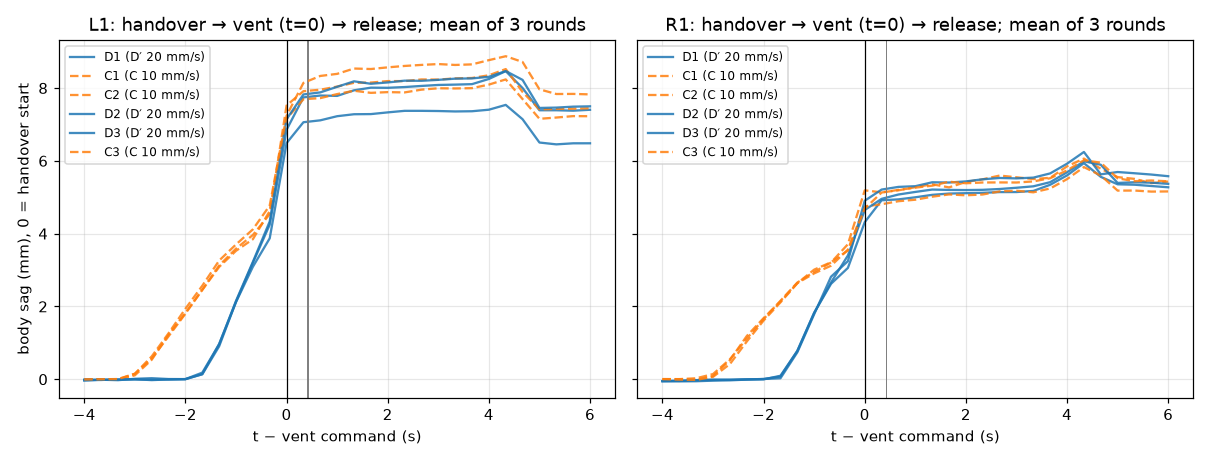
\includegraphics[width=\linewidth]{figures/dprime_profile.png}
\caption{判别结果的直观呈现:全六组交接剖面按放气指令($t{=}0$)
对齐,逐腿轮均值(左 L1,右 R1)。转移速率翻倍后(D$'$,实线)下沉
斜坡比对照(C,虚线)陡一倍,但终点\emph{平台相同}——下沉跟随转移的
毫米数,不随耗时。\TODO{按其他插图统一风格重制(字体/配色);当前为
分析报告原图}。}
\label{fig:dprime}
\end{figure}

\subsection{代价}
\label{sec:cost}

交接把冲击式损失换成舵机持续扛载:整组电流增量从 $+0.97\pm0.02$\,A
(A)升到 $+2.40\pm0.08$\,A(B),权重又收回到 $+1.85\pm0.08$\,A
(C,较 B $-23\%$——方向一致,约为模型 $-32\%$ 储能稀释的三分之二)。
周期时间增加转移时长($10$\,mm/s 下每步 $2.2$--$3.3$\,s)。两项都是
不加传感器的代价;第~\ref{sec:discussion} 节讨论这一权衡。

\subsection{偏差与效度威胁}
\label{sec:deviations}

我们记录全部偏差。(i)~一组录像开晚,裁掉对时标记;最初的后备对时
(对周期性阶跃模式做回归)锁错一个周期、逐腿归因错位;错误因逐腿模式的物理
不可能而被察觉,改用容忍裁剪的标记拟合重新对时($R^2=0.99$,幅值与
其余八个标记独立互证),修正后该组与全部交叉检验一致。教训已固化进
管线:用阶跃对时前先核实阶跃周期性;$60$\,s 起跑静置已内建进启动序列。
(ii)~三场中有两场相机在组间动过(\#1 A$\to$B 约 $128$\,px、\#2
C$\to$A 数十 px),组内从未:比例本就逐组标定,组内漂移由静物参照补偿
($\le4.8$\,px)。(iii)~场内各组间未回充电池
($7.5$--$8.1$\,V 区间);拉丁方使其与条件解耦。(iv)~NCC 模板得分
中位(主实验 $0.39$--$0.76$,D$'$ 系列 $0.70$--$0.86$)在板面倾斜的组
低于内部 $0.8$ 标准;参照块得分
($\ge0.988$)与九组互证(CV $1.6$--$4\%$)约束了影响。(v)~比例
参考机身板平面;顶/底边不一致($1.1$--$2.7\%$)约束残余透视误差。
(vi)~D$'$ 系列有两组,每次交接约 ${\sim}1$\,mm 的弛豫尾巴越过交接/vent
分段边界,在相邻两列之间挪动约 $4$--$5$\,mm/组;合并段与总量不受
影响。以上没有一项接近效应量级
($43$--$88\%$)。

% =========================================================================
\section{讨论}
\label{sec:discussion}

\emph{柔性是不是设计缺陷?}柔性不是可以简单设计掉的制造缺陷:
轻量打印腿、波纹吸盘、无传感齿轮系是几公斤级爬壁机的常规构造,而失效组合的每一要素——柔性支撑链、破裂型脱附、位置域
驱动——在整个平台类别中反复出现(第~\ref{sec:related} 节)。分析
在解法之外多给出一条设计准则:可补偿性受支撑集刚度谱约束。
对最硬的腿,任何权重都无法把 \eqref{eq:redistribution} 的再分配项
消零(把份额全给 R1,L1 的归一化系数仍有 $0.038$,按 $\delta=31$\,mm
折合每次 L1 交接约 $1.4$\,mm)——想只靠软件管理脱附的设计者,
应当约束的是各腿刚度的\emph{散布},而不只是水平。反过来,由于该解法
是约 $150$ 行、零硬件的软件改装,它可以不加修改地部署到现有的位置
控制爬壁机上。

\emph{为何开环而不用电流反馈?}这个选择基于数据。整机电流无法逐腿
归因:卸载硬腿时,总电流的平台拐点是卸载/接载增益的平衡点、不是零力点
(在一个电流看似已收敛的剂量下该腿仍弹跳 $6.9$\,mm);卸载软腿时总
电流单调上升——没有可用的反馈信号。逐腿力传感正是我们要避免的硬件;
电机电流估力
\cite{wahrburg2018motor} 需要业余齿轮系不遵守的摩擦模型。与此同时,
开环表免估计、免调参,且——如 $n{=}3$ 的散布所示(相对效应重复间
差 $5$ 个百分点以内)——跨天稳定无需重标。自然的闭环升级是事件式
而非连续式:破裂瞬间的电流台阶(乃至 IMU 脉冲)正比于残余储能,
可让机器人在两次爬行之间自校 $\delta$ 表;我们刻意把它留作后续,
使当前结果立足于不加任何传感器之上。

\emph{以模型门控实验选择。}拟合模型排除了我们计划中的一个条件:
刚度感知份额(选 $w_i$ 逐腿消零 \eqref{eq:redistribution})只动
再分配项,值 $3$--$4$\,mm,不值得为此做一次上墙实验。它也正确预测了
速率干预的结果,两种解读事先都已写定。要求模型在每次实验前给出预测
数字,这一做法与任何单项结果同样有价值。

\emph{推广与局限。}现象需要三个要素:锚点与机体之间的串联柔性、比
支撑系再平衡更快地释放接触的脱附方式、以及跟踪位置而非力的驱动。
任意光滑表面上的真空吸盘都满足;定向干粘附基本不满足(按设计剥离,
近零力释放 \cite{autumn2006frictional,kim2008smooth}),因此这一
问题在仿壁虎爬壁机上不会出现。我们的证据是一台平台、一种表面、一个
原地代理任务、三轮、$n{=}3$:效应很大且内部自洽,但绝对刚度(挂重
标定)、开着交接的净前进爬行、更长轮数(\eqref{eq:fit} 的轮增长因子 $\gamma$ 与 \eqref{eq:kappa}
中的 $0.20$ 在 $r{=}3$ 尚未饱和)、以及 $\kappa$ 的微观机理(它取决于
份额有多集中、还是取决于接载吸盘吸附了多久,可由份额扰动实验分离)
仍然开放
\TODO{T4a/T4b 结果出来后并入}。$\delta$ 表是开环标定:载荷或姿态
超出标定工况需重跑三剂量流程(一场)或采用上述事件式自校。

% =========================================================================
\section{结论}

每一台离散步态的吸附爬壁机,都会在密封断开的那一刻损失位置。在一台
柔性、位置控制的六足上,我们精确测量了这一损失——每周期 $64$\,mm 原地
下滑的 $93\%$ 压缩在破裂后的毫秒之内——把它溯源到机器人自重在腿链
中储存的弹性能,并说明了直觉的补救——放慢放气——为何无济于事:力在
唇口剥离的一瞬一次释放,而不是随压力衰减逐渐释放。
因为吸附的脚不会滑,补救可以完全在足端指令中实现:放气之前归还每条腿的
储存变形,把载荷在均值不变、轮转加权的份额下移交给其余腿,密封断开
时便无可释放。不用力传感、零新硬件、一次离线标定,棘轮的破裂分量下降
$88\%$、总量下降 $61\%$;剩下的部分服从一条简单的逐毫米转移定律,
其系数由载荷份额分配决定——这是我们下一步的工作目标。

% =========================================================================
\section*{多媒体附件}
\TODO{投稿必备视频:A vs C 原地并排 $+$ 单次破裂 30\,fps 慢放;MOV
原片冻结于实验机;若转投会议须 $\le$20\,MB/180\,s。}

\section*{数据可用性}
\TODO{开源包:九组 $+$ 六组日志、轨迹与分解报告、188 张核对图、分析
管线(追踪/对时/分解/拟合)、$\delta$ 标定协议。定托管处与许可证。}

\bibliographystyle{IEEEtran}
\bibliography{refs}

\end{document}
